\documentclass[
  a4paper,
  emulatestandardclasses,
  abstract,
  parskip,
  appendixprefix,
  listof=totoc,
  bibliography=totoc
]{scrreprt}

\usepackage[ngerman,english]{babel}

\usepackage{bm}
\usepackage{xcolor}
\usepackage{a4wide}
\usepackage{authblk}
\usepackage{physics}
\usepackage{amsthm}
\usepackage{amsmath}
\usepackage{amssymb}
\usepackage{csquotes}
\usepackage{caption}
\usepackage{biblatex}
\usepackage{enumerate}
\usepackage{graphicx}
\usepackage{hyperref}
\usepackage{cleveref}
\usepackage[
  binary-units
]{siunitx}
\usepackage[
  acronym,
  nonumberlist,
  toc,
  nohypertypes={acronym}
]{glossaries}
\usepackage{unicode-math}

\addbibresource{literature.bib}

\makeglossaries
\newacronym{rf}{RF}{radio frequency}
\newacronym{sma}{SMA}{SubMiniature version A}
\newacronym{smf}{SMF}{single-mode optical fiber}
\newacronym{aom}{AOM}{acousto-optic modulator}
\newacronym{aod}{AOD}{acousto-optic deflector}
\newacronym{dds}{DDS}{direct-digital synthesizer}
\newacronym{ccd}{CCD}{charge-coupled device}
\newacronym{ic}{IC}{integrated circuit}
\newacronym{pll}{PLL}{phase-locked-loop}
\newacronym{ad9910}{AD9910}{direct-digital synthesizer from Analog Devices}
\newacronym{asf}{ASF}{amplitude scale factor}
\newacronym{ftw}{FTW}{frequency tuning word}
\glsaddall

\subject{Many Body Quantum Optics}
\title{High-precision time-averaged optical potentials for ultracold atoms}
\subtitle{Bachelor thesis by}
\author[1]{Bodo Kaiser}
\affil[1]{Ludwig-Maximilians-Universität München}
\affil[ ]{\textit{bodo.kaiser@physik.uni-muenchen.de}}
\publishers{originated under the supervision of Prof. Dr. Immanuel Block,\\
  Dr. Monika Aidelsburger and Christian Schweitzer.}

\begin{document}

\makeatletter
\begin{titlepage}
  \begin{center}
    \usekomafont{subject}
    \@subject

    \vspace{.8em}
    \usekomafont{title}\huge
    \@title

    \vspace{.5em}
    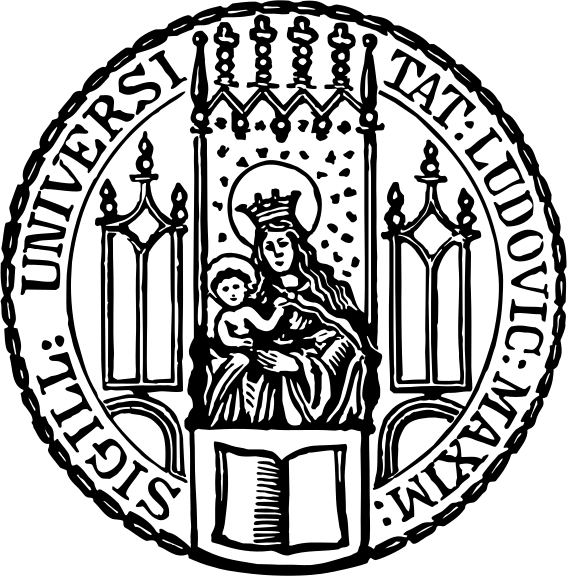
\includegraphics[width=.5\pagewidth]{build/emblem.pdf}

    \usekomafont{subtitle}
    \@subtitle

    \vspace{.8em}
    \usekomafont{author}
    \@author

    \usekomafont{date}
    \@date

    \vspace{.8em}
    \usekomafont{publishers}
    \@publishers
  \end{center}
\end{titlepage}
\makeatother

\makeatletter
\begin{titlepage}
  \begin{otherlanguage}{ngerman}
    \begin{center}
      \usekomafont{subject}
      Mehrteilchen Quantenoptik

      \vspace{.8em}
      \usekomafont{title}\huge
      Hochpräzise zeitgemittelte optische Potentiale für ultrakalte Atome

      \vspace{.5em}
      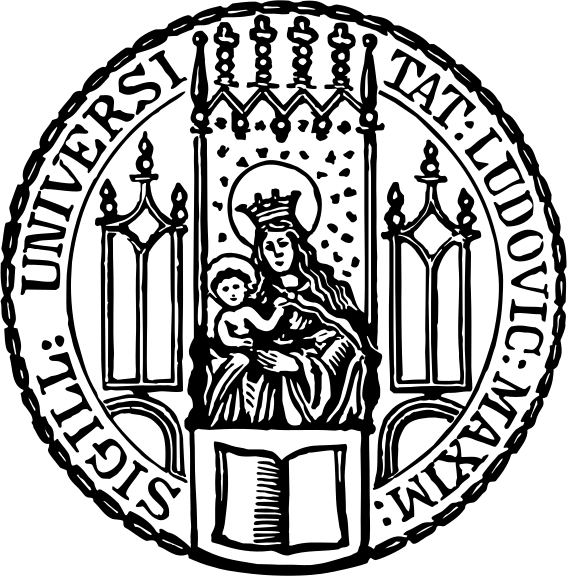
\includegraphics[width=.5\pagewidth]{build/emblem.pdf}

      \usekomafont{subtitle}
      Bachelorarbeit von

      \vspace{.8em}
      \usekomafont{author}
      \@author

      \usekomafont{date}
      \@date

      \vspace{.8em}
      \usekomafont{publishers}
      entstanden unter der Betreuung von Prof. Dr. Immanuel Block,\\
      Dr. Monika Aidelsburger und Christian Schweitzer.
    \end{center}
  \end{otherlanguage}
\end{titlepage}
\makeatother

\addchap{Acknowledgement}

The success and final outcome of the present work required a lot of guidance
and assistance from many people, without them it would not have been possible
for me to deliver this piece of work and look back on to the exciting,
enriching and diverse experience made in the last weeks, and I would not
forget to thank them.

At most I want to thank my parents for their support, that I have been
privileged to benefit from all the years. Though my life involved many
unexpected turnarounds, I never felt left alone and could rely on your
diverse experience.

Further I want to thank Prof. Bloch and Dr. Aidelsburger for creating and
sustaining a fertile scientific environment that allows inspiring discussions
at almost any time as well as seamless implementation of new ideas. Equally I
want to express my gratitude to all personal involved in the formation process
of my thesis. Especially I want to name Christian Schweizer, Hendrik v. Raven
and Till Klostermann who were available for any questions but also open to
fun from time to time. Finally I want to thank Bodo Hecker for any electronic
specific advise.

I also owe my deep gratitude to XY, who have been so friendly to check this
thesis against all sort of language abuses and offer a wide range of
suggestions to improve the expressiveness.

\addchap{Declearation of Authorship}

\addsec{Statutory Declearation}

I hereby declare that this thesis has been composed solely by myself except
where indicated otherwise by reference or acknowledgment.

The work presented has not been submitted, in whole or in part, in any
previous application for a degree.

\vspace{1em}
\textbf{Munich, \today}

\begin{abstract}
Lorem ipsum dolor sit amet, consectetur adipisici elit,
sed eiusmod tempor incidunt ut labore et dolore magna aliqua. Ut enim ad
minim veniam, quis nostrud exercitation ullamco laboris nisi ut aliquid ex ea
commodi consequat. Quis aute iure reprehenderit in voluptate velit esse
cillum dolore eu fugiat nulla pariatur. Excepteur sint obcaecat cupiditat
non proident, sunt in culpa qui officia deserunt mollit anim id est laborum.
\end{abstract}


\tableofcontents

\chapter{Introduction}

Many quantum systems studied in condensed matter physics are experimentally
challenging to access as any interactions can destroy the carefully prepared
quantum states. As way forward, experiments with ultracold atoms in
optical lattices give us a highly contorllable environment, giving us the
opportunity to simulate and explore quantum effects and expand our current
understanding of quantum mechanics and statistical physics \cite{Gross2017}.

The central idea behind these types of experiments is to cool down neutral
atoms to micro Kelvin and below, and load them into an optical lattice. At
these temperatures atoms demonstrate quantum behaviour. The optical lattices
act as periodic potentials analogue to the periodic potential found inside
solid state crystal lattices \cite{Lewenstein2007}. Unlike to i.e. real solids
where we have limited prospects to amend a systems properties, lasers driven
by state of the art optics and electronics give us a wide range of well
controllable parameters.

\begin{figure}[h]
  \centering
  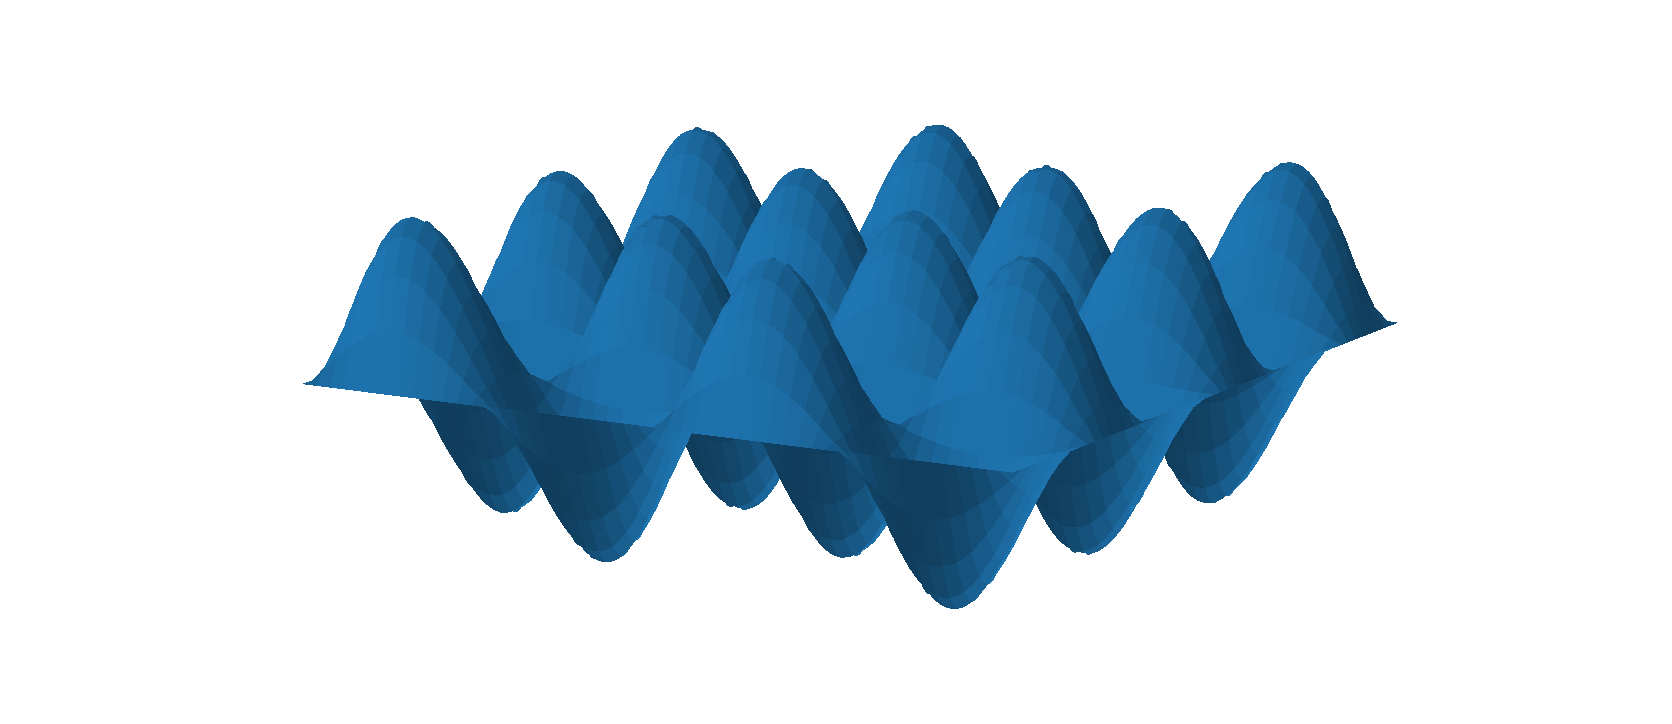
\includegraphics[width=.8\textwidth]{images/optlat/default.pdf}
  \captionsetup{width=.8\textwidth}
  \caption{Periodic potential of a 2D optical lattice. If the kinetic energy
  of the atoms is below the potential energy of the lattice, the atoms will
  locate around the potential minimas.}
  \label{fig:optlat}
\end{figure}

One of the parameters of interest is the ability to apply local potentials
to the system, that can be used to, among others, study lattice inpurities
or quantum interactions. In this work we will present and characterize one
possible implementation of such a local potential generating apparatus.

\section{Related Work}

Local manipulations of atoms inside optical lattices have been known for some
time in the embodiment of optical tweezers that allow trapping, stacking and
sorting of particles \cite{Tadmor2004}. Yet, only recently attempts to
interact with local particle clusters through high-precision time-averaged
optical potentials have been reported \cite{Roy2016}.

In the following we continue on the laid out work \cite{Hertlein2017} which
provided us with an optical setup for single-site manipulation using
\gls{aod} as well as considerations with regard to aperture limited
gaussian beam propagation.

\chapter{Theory of Optical Lattices}

In this chapter we will recapitulate the theoretical foundations of optical
lattices used in ultracold quantum experiments, thereof we can derive
theoretical requirements for the planned potential generation. Most notably
we are interested in the domain of the sweep duration and resolution that
our setup has to operate in.

\section{General Case}

\subsection{Periodic Potentials}

The Schrödinger equation of a particle state $\ket{\Psi}$ subject to a time
independent one-dimensional potential reads
\begin{align}
  E\ket{\Psi}
  =\hat{H}\ket{\Psi}
  =\left(\frac{\hat{p}^2}{2m}+\hat{V}\right)\ket{\Psi}
  \label{eq:time_independent_schroedinger}.
\end{align}
For a periodic potential $V(x+a)=V(x)$ the Bloch-Theorem \cite{Ashcroft1976}
states that the wavefunction of a particle in a periodic potential can be
written as
\begin{equation}
  \braket{\hat{x}}{\Psi}
  =\Psi(x)
  =e^{iqx}\psi(x)
  \label{eq:bloch_theorem}
\end{equation}
wherein $-\frac{\pi}{a}<q<+\frac{\pi}{a}$ is the quasimomentum, a quantum
number characteristic of the translational symmetry of the periodic potential
\cite[p. 42]{Lewenstein2012} with $a$ being the lattice constant.

The momentum operator is a differential operator in position space
\begin{equation}
  \hat{p}
  =\expval{\hat{p}}{\hat{x}}
  =-i\hbar\dv{x}
  \label{eq:momentum_operator_in_position_space},
\end{equation}
thus we obtain $\hat{p}e^{iqx}=\hbar qe^{iqx}$ and
$\hat{p}^2\ket{\Psi}=e^{iqx}\left(\hat{p}+\hbar q\right)^2\ket{\psi}$ such
that we can rewrite \cref{eq:time_independent_schroedinger} for
the periodic case
\begin{equation}
  E\ket{\psi}
  =\left(\frac{(\hat{p}+\hbar q)^2}{2m}+\hat{V}\right)\ket{\psi}
  =:\hat{H}_{periodic}\ket{\psi}
  \label{eq:periodic_schroedinger}.
\end{equation}

Translational symmetry of the potential enforces discrete particle momenta
$p_n=pn=nk\hbar$ such that we can represent our particle state in a
countable momentum basis
\begin{equation}
  \ket{\psi}
  =\mathbb{1}\ket{\psi}
  =\left(\sum_n\ket{p_n}\bra{p_n}\right)\ket{\psi}
  =\sum_n\braket{p_n}{\psi}\ket{p_n}
  =\sum_nc_n\ket{p_n}
  \label{eq:countable_momentum_state}.
\end{equation}
Inserting this into the right hand side of \cref{eq:periodic_schroedinger}
yields us
\begin{equation}
  \hat{H}_\text{periodic}\ket{\psi}
  =\sum_nc_n\left(\frac{(\hat{p}+\hbar q)^2}{2m}+\hat{V}\right)\ket{p_n}
  =\sum_nc_n\left(\frac{(pn+\hbar q)^2}{2m}+\hat{V}\right)\ket{p_n}
  \label{eq:periodic_hamiltonian_in_momentum_base}
\end{equation}
where we used the eigenvalue equation $\hat{p}\ket{p_n}=pn\ket{p_n}$ to
satisfy the second equal sign. By applying an orthogonal $\bra{p_m}$ to the
left hand side of \cref{eq:periodic_hamiltonian_in_momentum_base} we find
the matrix elements of the periodic Hamiltonian
\begin{equation}
  \hat{H}_{\text{periodic},mn}
  =\mel**{p_m}{\hat{H}_\text{periodic}}{p_n}
  =(m+q/k)^2\frac{\hbar^2k^2}{2m}+\mel**{p_m}{\hat{V}}{p_n}
  \label{eq:periodic_hamiltonian_elements}
\end{equation}
where we used $p=\hbar k$ in the last step.

Usually the potential will be known in position space. Through use of the
completeness relation
\begin{equation}
  \mathbb{1}
  =\int\dd{x}\op{x}{x}
  \label{eq:continous_completeness_relation}
\end{equation}
we are able to transform the potential in momentum space
\begin{equation}
  V(p)
  =\mel**{p_m}{\hat{V}}{p_n}
  =\int\int\dd{x}\dd{y}\braket{p_m}{x}\mel**{x}{\hat{V}}{y}\braket{y}{p_n}
  =\int\frac{\dd{x}}{\sqrt{2\pi\hbar}}e^{ikx(m-n)}V(x)
  \label{eq:potential_fourier_transform}.
\end{equation}
after the identification of $\braket{p}{x}=e^{ipx/\hbar}/\sqrt{2\pi\hbar}$.

\subsection{Harmonic Potentials}

In the former section we discussed the quantum mechancis of a generic
periodic potential. We will now consider the special case of a harmonic
potential of the shape
\begin{equation}
  V(x)
  =V_0\cos^2(kx)
  =\frac{1}{4}V_0\left(e^{+2ikx}+e^{-2ikx}+2\right)
  \label{eq:harmonic_potential}.
\end{equation}
Potentials of such form can be found for example in the standing wave of a
reflected gaussian beam
\begin{equation}
  V(r,x)
  =V_0e^{-2r^2/w(x)^2}\cos^2(kx)
  \approx V_0\cos^2(kx)
  \label{eq:optical_potential}
\end{equation}
wherein $r$ denotes the beam radius, $w(x)$ being spot size parameter and
$k=2\pi/\lambda$ with the laser wavelength $\lambda$. The approximation is
valid for $w(x)\gg r$ which holds in most cases according to
\cite[p.127]{Rom2009}.

Transformation of \cref{eq:harmonic_potential} to momentum space
using \cref{eq:potential_fourier_transform} yields
\begin{equation*}
  V(p)
  =
  \frac{1}{4}V_0
  \int\frac{\dd{x}}{\sqrt{2\pi\hbar}}
  e^{+ipx(m-n)/\hbar}\left(e^{+2ikx}+e^{-2ikx}+2\right)
  =
  \frac{1}{4}V_0\left(2\delta_{m,n}+\delta_{m,n+2}+\delta_{m,n-2}\right).
\end{equation*}
The Hamiltonian \cref{eq:periodic_hamiltonian_elements} of a
harmonic potential then reads
\begin{equation}
  \hat{H}_\text{harmonic}
  =\begin{cases}
    (n+q/k)^2\frac{\hbar^2k^2}{2m}+\frac{1}{2}V_0, & \text{if } n=m\\
    \frac{1}{4}V_0, & \text{if } \abs{n-m}=2\\
    0, & \text{otherwise}
  \end{cases}
  \label{eq:harmonic_hamiltonian}.
\end{equation}
Plotting the eigenvalues of \cref{eq:harmonic_hamiltonian} against
$q$ we find the characteristic energy band structure giving us the allowed
energy ranges.

In the case of optical potentials. We would further introduce the recoil
energy $E_r=(\hbar k)^2/(2m)$ which gives us a natural atom independent scale
to work with.

\section{Free-Particle Approximation}

In the free-particle approximation we consider flat potentials or particles
with higher kinetic than potential energy. In this regime energy gaps
vanish and particles can move freely. For the present work this is not
relevant circumstance as particles as local potentials we are interested
to generate onto the existing lattice structure would just move around
particles.

\section{Tight-Binding Approximation}

In the tight-binding approximation the potentials are considered deep or
particles to have lower kinetic than potential energy, such that interaction
between neighbooring particles is limited. In the optical case potentials can
be easily made deep by increasing the intensity. In this regime energy bands
converge to discrete energy levels with inbetween energies being forbidden.

\subsection{Periodic Potentials}

\subsection{Harmonic Potentials}

\chapter{Theory of Acousto-Optics}

\section{Light Interaction}

\section{Piezoelectric Transducer}

\chapter{Theory of Digital Signal Synthesis}

\section{Phase Accumulator}

\section{Lookup Table}

\section{Operating Range}

We apply a reference signal of
\begin{equation}
  f_\text{ref}=\SI{10}{\mega\hertz}
\end{equation}
configured to be used with a \gls{pll} multiplier of
$N=100$ yielding a system clock of
\begin{equation}
  f_\text{sys}=Nf_\text{ref}=\SI{1}{\giga\hertz}.
\end{equation}
The timer clock used for the linear ramp and memory playback runs with
a quarter of the system clock
\begin{equation}
  f_\text{timer}=f_\text{sys}/4=\SI{250}{\mega\hertz}.
\end{equation}

The \gls{ad9910} uses a \SI{14}{\bit} \gls{asf} and \SI{32}{\bit} \gls{ftw}
to parameterize amplitude $A(t)$ and output frequency $f(t)$ by
\begin{align}
  FTW
  :=
  \left\lfloor2^{32}\left(\frac{f_\text{out}}{f_\text{sys}}\right)\right\rceil
  &&
  ASF
  :=
  \left\lfloor\frac{A_\text{out}}{2^{14}}\right\rceil
  \label{eq:elec:ftwasf}
\end{align}
wherein $\lfloor{\cdot}\rceil$ rounds the given float to the nearest integer.
The theoretical limit for the maximum output frequency then is found via
\begin{equation*}
  f_\text{max}
  =
  \left(1-\frac{2^{31}-1}{2^{32}}\right)f_\text{sys}
  =
  \left(\frac{1}{2}-\frac{1}{2^{31}}\right)f_\text{sys}
  \approx
  \frac{1}{2}f_\text{sys}
  =
  \SI{500}{\mega\hertz}.
\end{equation*}
Yet the datasheet \cite{AD9910} reports $f_\text{max}=\SI{420}{\mega\hertz}$
and in fact we found the output signal to be very noisy at the theoretical
limit.

We continue with the assessment of the digital ramp that does a unidrectional
linear sweep on the frequency from \SI{90}{\mega\hertz} to
\SI{110}{\mega\hertz}. The digital ramp of the \gls{ad9910} lets us define
a \gls{ftw} step $M$ word of \SI{32}{\bit} as well as a step rate word $S$ of
\SI{16}{\bit} resolution. They relate to the frequency step and the time
step through
\begin{align}
  \Delta f
  =
  \frac{M}{2^{32}}f_\text{sys}
  &&
  \Delta t
  =
  \frac{S}{f_\text{timer}}
  =
  \frac{S}{4f_\text{sys}}.
  \label{eq:elec:step}
\end{align}
The sweep duration is deterimened by $S,M$ through
\begin{equation}
  T_\text{duration}
  =
  \frac{f_\text{upper}-f_\text{lower}}{\Delta f}\Delta t
  =
  2^{32}\frac{f_\text{upper}-f_\text{lower}}{f_\text{sys}}\frac{S/M}{f_\text{timer}}
\end{equation}
for a target sweep duration of $T_\text{duration}=\SI{10}{ms}$ we find
\begin{equation*}
  \frac{S}{M}
  =
  \frac{T f_\text{timer}}{2^{32}}\frac{f_\text{sys}}{f_\text{upper}-f_\text{lower}}
  =
  \frac{10^9}{2^{35}}
  \approx
  \num{2.9104e-2}
  =
  \frac{1819}{62500}
\end{equation*}
the last step can be obtained by best ratio approximation using continued
fractions as for example described in \cite{Ashley2003}. It should be kept in
mind that the best ratio approximation is likable to introduce an error,
therefore realistic durations may differ from the configured value and it
is possible that better approximations exist that allow smaller $\Delta f,
\Delta t$, thus providing a sweep resolution. In the above case the given
time duration translates to
\begin{align*}
  \Delta f
  =
  \frac{62500}{2^{32}}f_\text{sys}
  \approx
  \SI{145}{\kilo\hertz}
  &&
  \Delta t
  =
  \frac{1819}{f_\text{timer}}
  \approx
  \SI{7.28}{\micro\second}
\end{align*}
or $(f_\text{upper}-f_\text{lower})/\Delta f=138$ discrete data points.

Eventually we are left with the assessment of the amplitude sequence. The
memory fits at most 1024 discrete amplitude values and the \gls{ad9910}
allows us to set the time spent at each amplitude value via the \SI{16}{\bit}
playback rate $P$ word
\begin{equation}
  \Delta t
  =
  \frac{P}{f_\text{timer}}
  =
  \frac{4P}{f_\text{sys}}
\end{equation}
which gives us range from $\min\Delta t=\SI{4}{\nano\second}$ to
$\max\Delta t=\SI{26.14}{\micro\second}$. As we incorporate all of the 1024
data points this gives us a duration range from about
$\min T=\SI{4}{\micro\second}$ to $\max T=\SI{26.84}{\milli\second}$.


\chapter{Experimental Setup}

The exerimental setup was largely adopted from \cite{Hertlein2017}, amendments
made include the \gls{rf} signal source of the \gls{aod} and an additional
photodiode to measure the deflected beam intensity.

\section{Optics}

The optical setup can be dissect into a closed first section that reduces
the power of the $\SI{532}{\nano\meter}$ laser source from $\SI{10}{\watt}$
to below $\SI{2}{\milli\watt}$ and an open second section for beam deflection.
Both sections are connected through a \gls{smf}.

\subsection{Power Reduction}
\label{sec:powerbox}

Because of safety concerns the power reduction section is confined into a
visually sealed superstructure. \Cref{fig:powerbox} reveals the inside of the
power reduction box.

\begin{figure}[h]
  \centering
  \includegraphics[width=\textwidth]{build/powerbox.pdf}
  \caption{Optical configuration of the power reduction section.}
  \label{fig:powerbox}
\end{figure}

The laser beam leaving the laser source is polarized by a $\lambda/2$ retarder
plate such that the succeeding high power beamsplitter BS can divert the
majority of the beams power into a high power beam dump.
Afterwards mirrors M1 and M2 direct the beam towards the center of a $2:1$
telescope composed of two lenses L1, L2 with focal lengths
$f_1=\SI{100}{\milli\meter}$ and $f_2=\SI{50}{\milli\meter}$.
An \gls{aom} diffracts the laser beam into multiple orders. Mirrors M3, M4
project theses orders onto a pinhole which is configured to intromit only the
the first order deflection. The intensity of the first order is subject to
amplitude modulation apllied to the \gls{aom}.
Finally a tunable $\lambda/2$ retarder plate can be used to couple the beam
polarization with the \gls{smf}.

\subsection{Beam Deflection and Detection}
\label{sec:deflection}

The section for beam deflection and detection as disclosed in
\cref{fig:deflection} receives the down-powered laser beam from previously
described section by a \gls{smf}. Hereinafter the beam passes a tunable
retarder plate and beam splitter BS1. The tunable retarder plate can be used
to adjust the beam intensity without having to access the power box.
A second polarizer with cube BS2 is used to branch off a part of the beam
to a photodiode PD1 that is positioned to be at the focal point of lens L1.
Photodiode PD1 is connected via a control system with the amplitude
modulation of the \gls{aom} depicted in \cref{fig:powerbox} to stabilize
the laser intensity against i.e. thermal drifts.

\begin{figure}[h]
  \centering
  \includegraphics[width=\textwidth]{build/deflection.pdf}
  \caption{Optical configuration of the beam deflection section.}
  \label{fig:deflection}
\end{figure}

For horizontal and vertical beam deflection two \gls{aod}s are used. A $1:1$
telescope comprised of two lenses L2, L3
each with focal length $f_2=f_3=\SI{250}{\milli\meter}$ projects the beam
on a pair of objectives that are built of lenses L4 to L7. The purpose of the
objective pair is to focus the laser on to the atom plane.
Consecutively the laser is reflected by a pair of mirrors M3 and M4 to the
part intended for detection. Lens L8 acts as a camera lens and projects the
beam to infinite focus on to the CCD camera sensor. Cube BS3 forks a portion
of the beam away from the CCD camera on to mirror M5 that guides the beam
towards lens L9 in order to focus the beam onto a second photodiode PD2.

\section{Electronics}

Beforehand we described the optical setups used. Now we want to emphasize
on the electronics how they are integrated into the optical setup.

\subsection{Signal Source}
\label{sec:elec:dds}

The requirements placed by the two \gls{aod} demand flexible but precise
\gls{rf} sources. Fortunately we can resort to a custom made signal
sources based on the \gls{ad9910} \gls{dds} \cite{AD9910} \gls{ic} that can
operate up to \SI{420}{\mega\hertz} and allows modulation of amplitude,
frequency and phase offset by either a constant value or through a single
digital ramp or playback from a memory sequence. Details on the working
principle of a simple \gls{dds} can be found in the \cref{app:elec:dds}.

The signal output of the \gls{dds} is of the form
\begin{equation}
  U(t)=A(t)\sin(2\pi f(t)+\phi(t)).
  \label{eq:dds:signal}
\end{equation}
In the following we will ignore the unsynced phase offset, thus setting
$\phi=0$. In case of the single \gls{dds} which drives the \gls{aom} we
have a constant signal, in that sense we can set $A=1$ and
$f_\text{aom}=\SI{80}{\mega\hertz}$ on \cref{eq:dds:signal}.
In the case of the two \gls{dds} which drive the horizontal and vertical
\gls{aod} we configure the frequency to be controlled by the digital ramp in
order to do a linear frequency sweep from
$f_\text{lower}=\SI{90}{\mega\hertz}$ to
$f_\text{upper}=\SI{110}{\mega\hertz}$, yielding
\begin{align}
  f_\text{aod}(t)
  =
  f_\text{lower} + \frac{f_\text{upper}-f_\text{lower}}{T_\text{duration}}t
\end{align}
wherein $T_\text{duration}>0$ denotes the sweep duration. The amplitude is
controlled by memory playback. Given a discrete set of amplitude values
$A_i\in[0,1]$ with $i=1,\dots,N=1024$ the amplitude of the \gls{aod} can be
formulated as
\begin{align}
  A_\text{aod}(t)
  =\sum^N_{i=1}A_i\mathbb{1}_{B_i}(t)
  &&
  B_i:=\left[iT_\text{interval}, (i+1)T_\text{interval}\right[
\end{align}
wherein $T_\text{interval}>0$ denotes the playback interval and
$\mathbb{1}_{B_i}$ is the characteristic function on the set $B_i$.

So far we have assumed $f_\text{aod}(t)$ to be continous and
$T_\text{interval},T_\text{duration}>0$ to be arbitrary, however the internals
of the \gls{ad9910} impose theoretical restrictions on the possible operating
ranges. For details we again want to refer to \cref{app:elec:dds}, here we will
only summarize the found limits.

\subsection{Signal Amplifier}

We use three signal amplifiers with respective input from the signal sources
to have an output power of about $P=\SI{2}{\watt}$ required by the \gls{aod}s
and \gls{aom} for ideal operation. The used amplifiers offer a second input
for external amplitude modulation. In case of the \gls{aom} we connect this
input with the intensity controller.

\subsection{Intensity Controller}

The intensity controller is connected to photodiode PD1 that converts the
laser intensity to an input voltage signal of the controller. Given the
input signal we can configure the controller for a reference input voltage.
The controller will then compare the input voltage with set reference voltage
and output an error signal that is proportional to the deviation of the
input from the reference voltage. The inverted error signal is feed to the
signal amplifier connected with the \gls{aom}.

In one attempt we tried to use the intensity controller to compensate for
frequency dependent intensity changes during frequency sweep of the \gls{aod},
however we found that even slow sweep times of $\SI{2}{\second}$ could not
be balanced, therefore the intensity controller only compensates for slow
intensity shifts caused by thermal stress of the laser source.

The intensity controller has to be connected correctly with photodiode PD1
of the setup as well as signal amplifier of the signal that drives the
\gls{aom}.

\begin{figure}[ht]
  \centering
  \includegraphics[height=6cm]{example-image-a}
  \caption{The intensity controller next to the \gls{aom} amplifier.}
  \label{fig:intcontrol}
\end{figure}

The XY can be tuned to set the reference signal.

\subsection{Trigger Source}

To syncronize the signal sources, the \gls{ccd} camera and the oscilloscope
it was necessary to design a global trigger source that outputs a rising edge
signal to multiple devices and exposes a network programable interface.

\begin{figure}[h]
  \centering
  \includegraphics[height=6cm]{example-image-a}
  \caption{The trigger source exposes a network programable interface and
  provides enough power to drive four output signals.}
  \label{fig:elec:trig}
\end{figure}

The schematics and board layout can be found in the \cref{app:elec:trigger}.

\section{Acousto-Optics}

\subsection{Modulator}

\subsection{Deflector}

\section{Calibration}

Alterations of the laboratory environment combined with the exchange of
components from the original setup made it necessary to recalibrate the setup.
In this chapter we want to document the calibration steps required to
reproduce the claimed results.

\subsection{Fiber Coupling}

The visually shielded section of the setup, used to reduce the output power
of the laser source, is optically paired with the open section for beam
deflection via a \gls{smf} that only permits two orthogonal polarization and
a single gaussian mode. By tuning the polarisator inside the power
reduction section we can try to match one of the orthogonal polarization
modes supported by the \gls{smf}. Polarization discrepancies cause the
polarization inside the \gls{smf} to oscillate with vibrations or changes in
temperature, henceforth it is key to couple polarization modes in order to
ensure a stable operation.

\begin{figure}[ht]
  \centering
  \includegraphics[height=6cm]{example-image-a}
  \caption{Intensity oscillations observed through the oscilloscope when
  heating the \gls{smf}.}
  \label{fig:fibercoup}
\end{figure}

A strategy proven to find an approximate polarization match between the
laser beam and the \gls{smf} is presented. In addition to the setup described
in \cref{sec:powerbox} and \cref{sec:deflection} an oscilloscope and a hot
air gun were used.

\begin{enumerate}
  \item Connect the photodiode to the oscilloscope and use a coarse time
    scale (i.e. \SI{2}{\second}).
  \item Apply appropriate laser safety glasses and inform present personal
    of the imminent danger.
  \item Open the cover of the power reduction setup.
  \item Apply heat to the \gls{smf} through the hot air gun, alternatively
    you can try to move the fiber.
  \item The photodiode signal should start to oscillate. Tune the polarizor
    inside the power reduction subject to minimizing the oscillation.
\end{enumerate}

The oscillations occur as the polarization circulates inside the fiber and
will stop at some point when a new equilbrium has been established. In this
case remove the heat or mechanical stress on the fiber and wait before you
reapplying new impetus.

\subsection{Beam Alignment}

Beams that pass off-centered through spherical lenses experience optical
aberrations, additionally uncentered beams may cause further optical defects
from reflections or clipping at boundaries. Since most changes to the optical
setup outdate the previous beam alignment, hence making the realignment
a rather frequent procedure, we want to showcase what worked well for us.

As auxilliaries we used a pair of iris diaphragms that can be placed in front
of the lens mounts as a screen (i.e. a white sheet of hard paper). By placing
both iris diaphragms towards the incident beam on two successive lenses we
we can visually find a center reference point by inspecting the symmetry of
the iris illumination at different pinhole diameters.

\begin{figure}[ht]
  \centering
  \minipage{0.45\textwidth}
    \includegraphics[width=\linewidth]{example-image-a}
    \caption{Typical beam alignment situation involving the mirrors M1, M2 and
    lenses L1, L2.}
    \label{fig:beamalign:setup}
  \endminipage
  \hfill
  \minipage{0.45\textwidth}
    \includegraphics[width=\linewidth]{example-image-a}
    \caption{Unaligned beam missing the iris pinhole and suggested mirror
    adjustments.}
    \label{fig:beamalign:iris}
  \endminipage
  \hfill
\end{figure}

\Cref{fig:beamalign:iris} shows a misaligned beam hits the iris diaphragms
and how to adjust the mirror angles. It should be noted that this is an
iterative process.

\subsection{Camera}

Finally we had to reposition the camera to focus the incoming beam on the
\gls{ccd} sensor of the camera. Finding the precise focus position is not an
easy undertaking. There is no sharp focal spot but rather a focal area,
however outside the focal area no image can be seen.

We followed the procedure described in \cite{Hertlein2017} that consists of
extracting the camera rail with its lens and focusing it on a far distant
object.

\begin{figure}[ht]
  \centering
  \minipage{0.5\textwidth}
  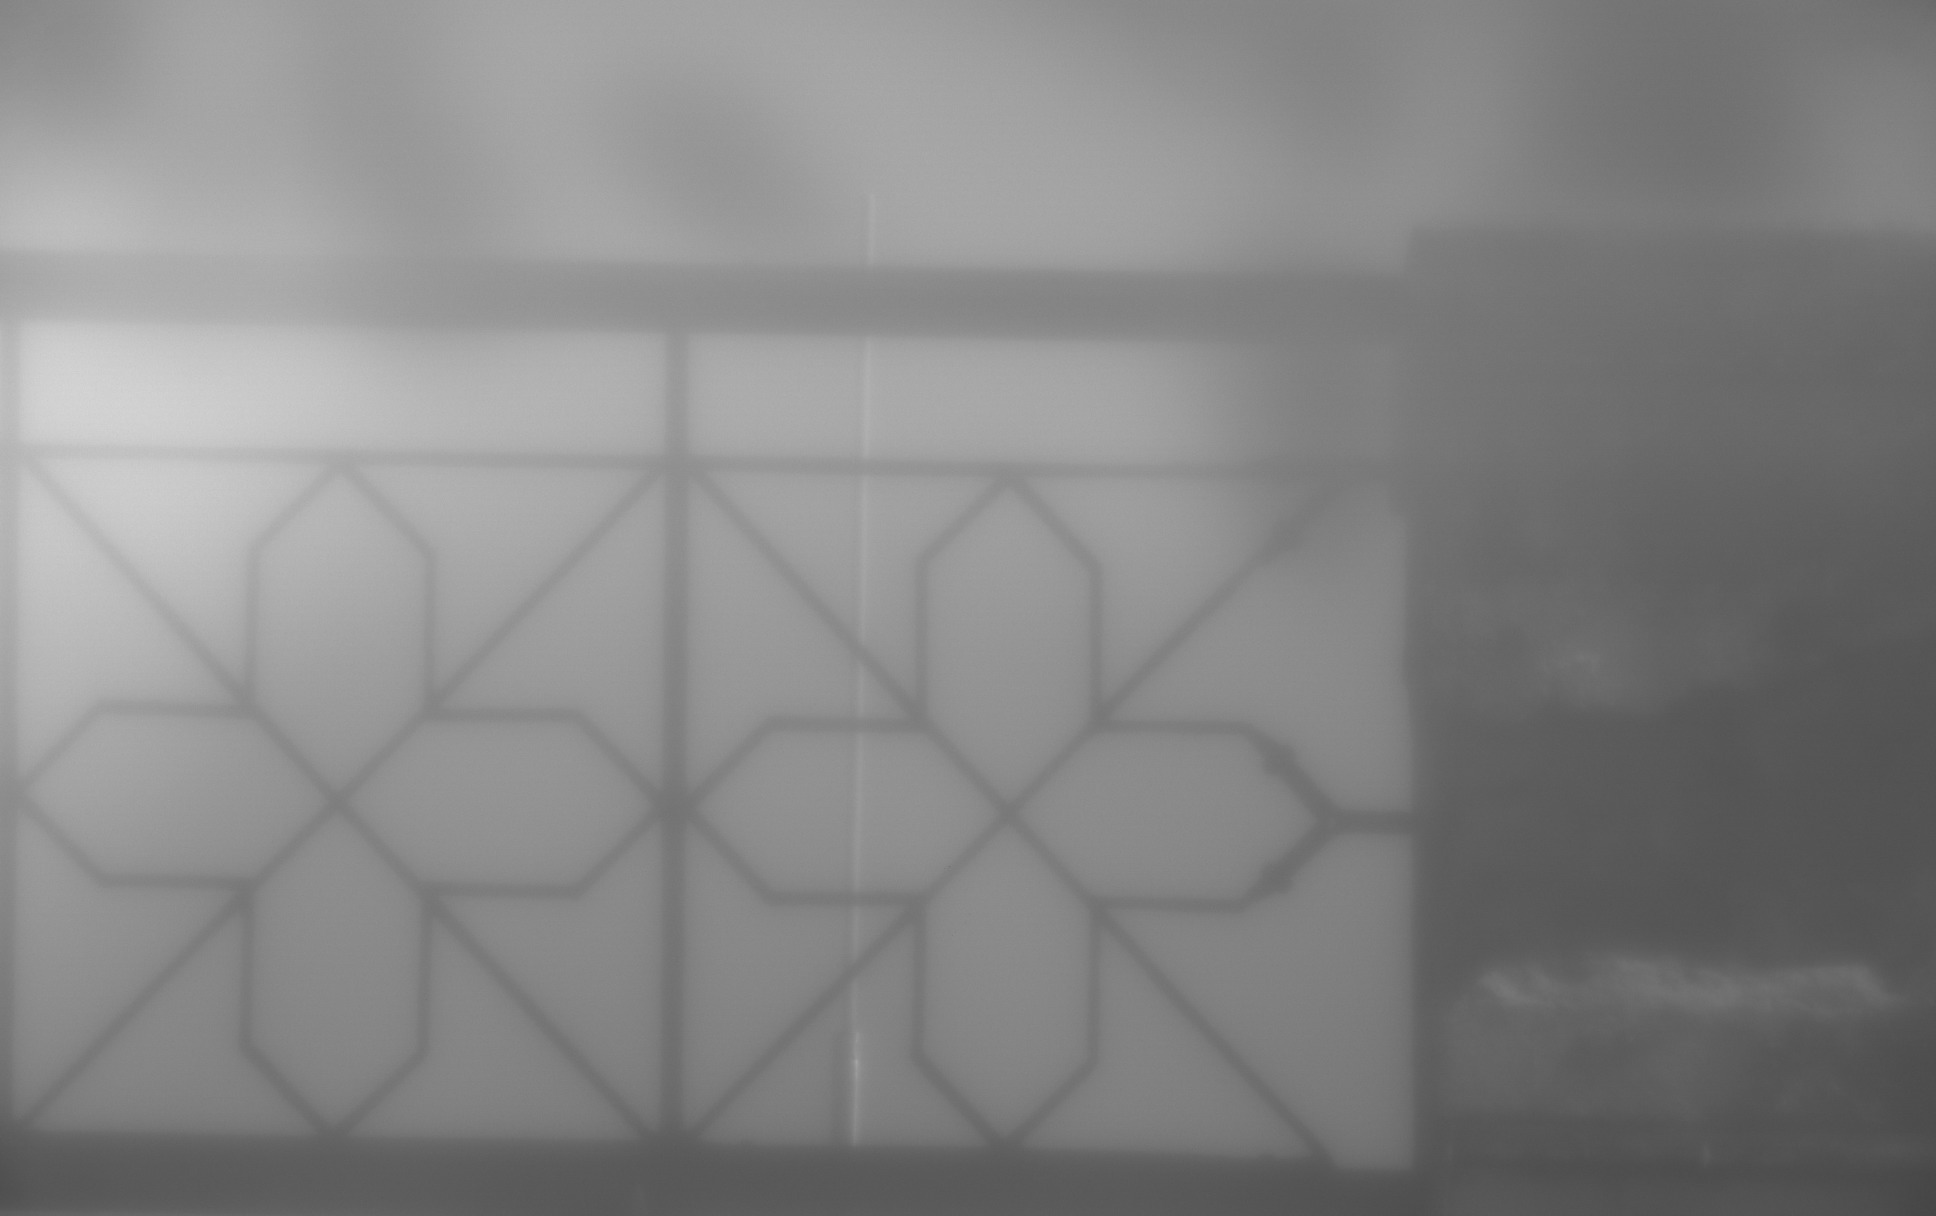
\includegraphics[width=\linewidth]{images/focus/focus2.jpg}
    \caption{Focused camera with view on the balcony bars on the top of the
    university tower.}
    \label{fig:camerafocus:balcony}
  \endminipage
  \hfill
  \minipage{0.45\textwidth}
    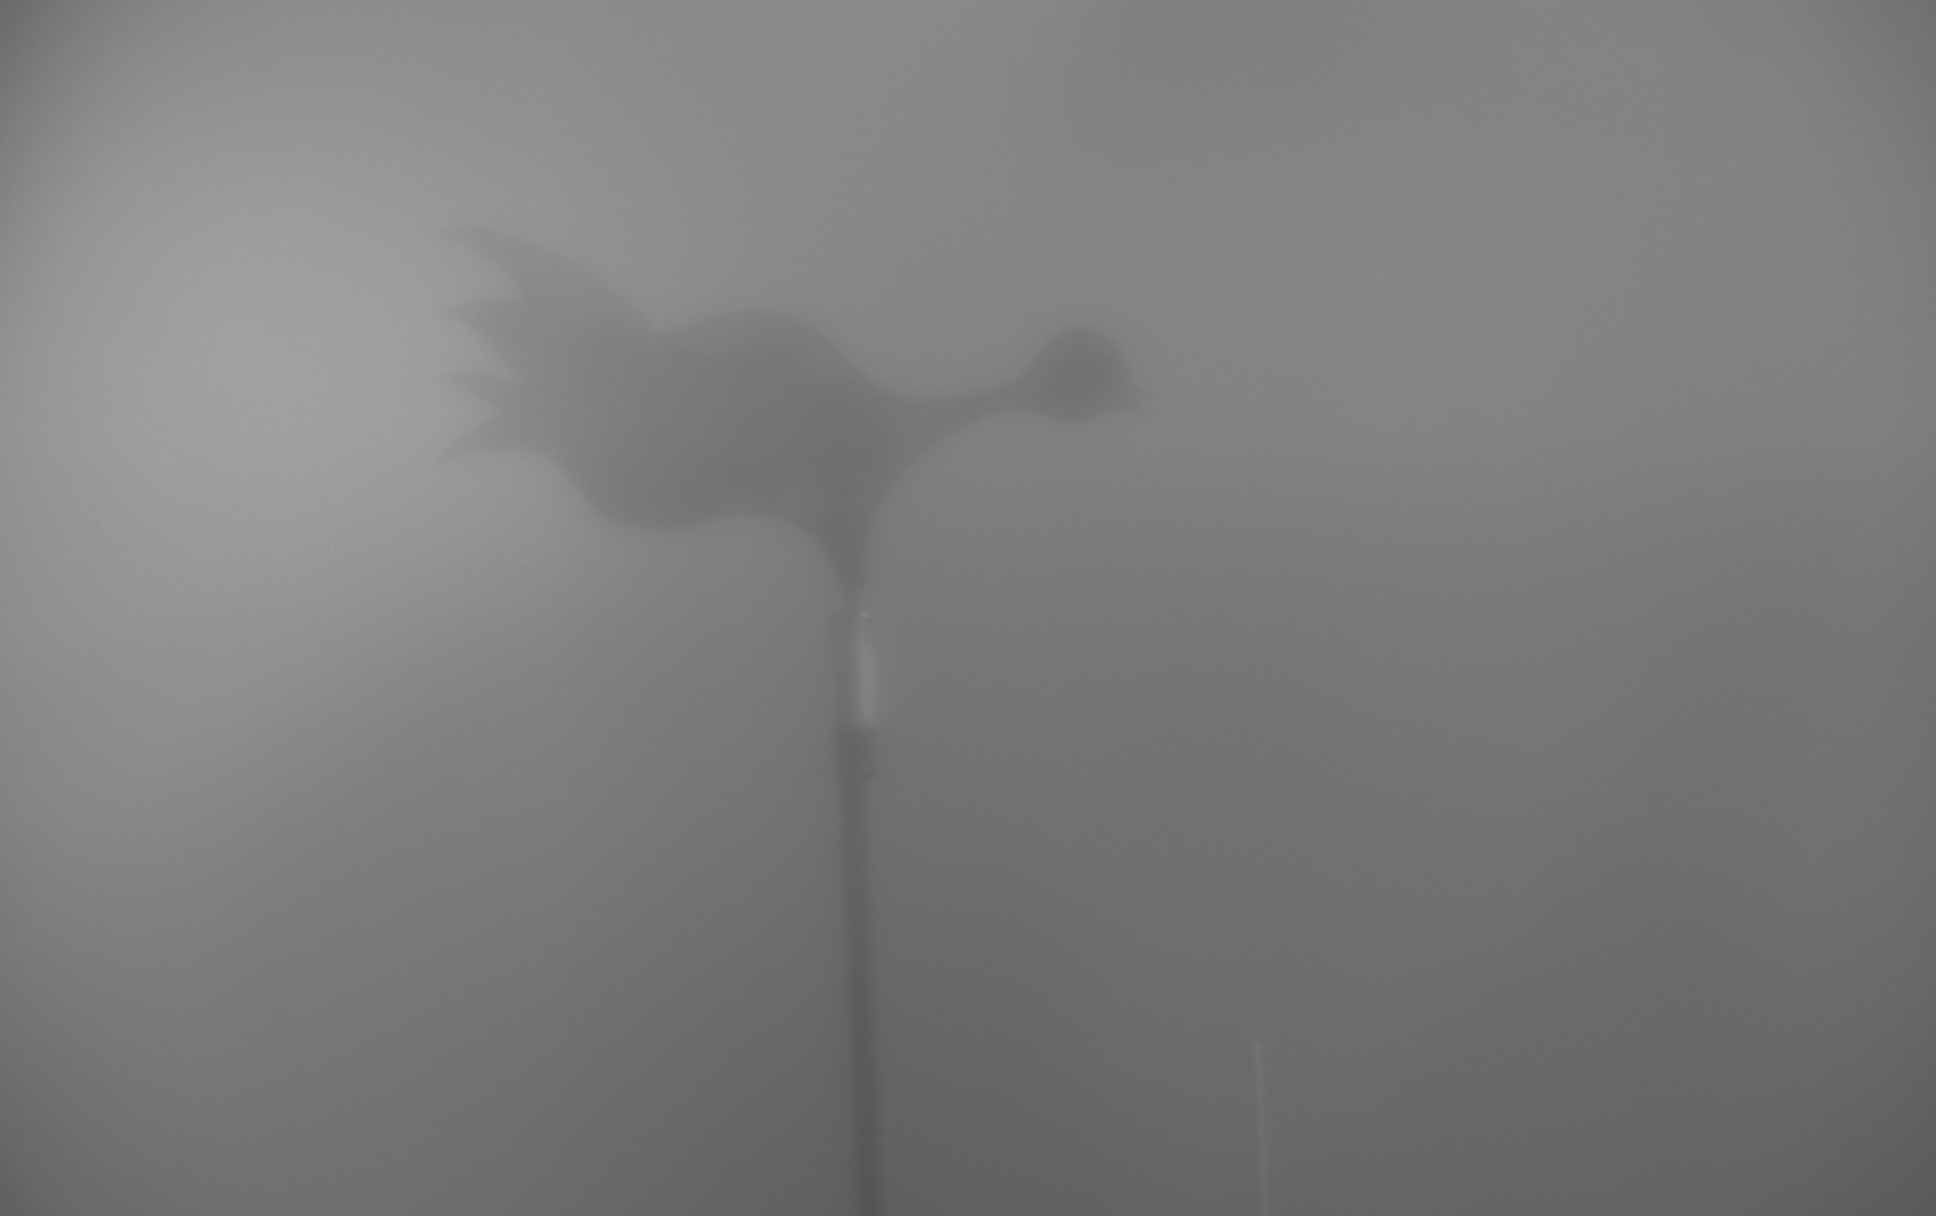
\includegraphics[width=\linewidth]{images/focus/focus3.jpg}
    \caption{Focused camera with view on the weather cock on the top of the
    university tower.}
    \label{fig:camerafocus:cock}
  \endminipage
  \hfill
\end{figure}

\section{Assessment}

With the previously described calibration steps in place we can assess the
final quality of the beam with an image capture of the \gls{ccd} camera in the
aligned setup \cref{sec:deflection}.

\begin{figure}[ht]
  \centering
  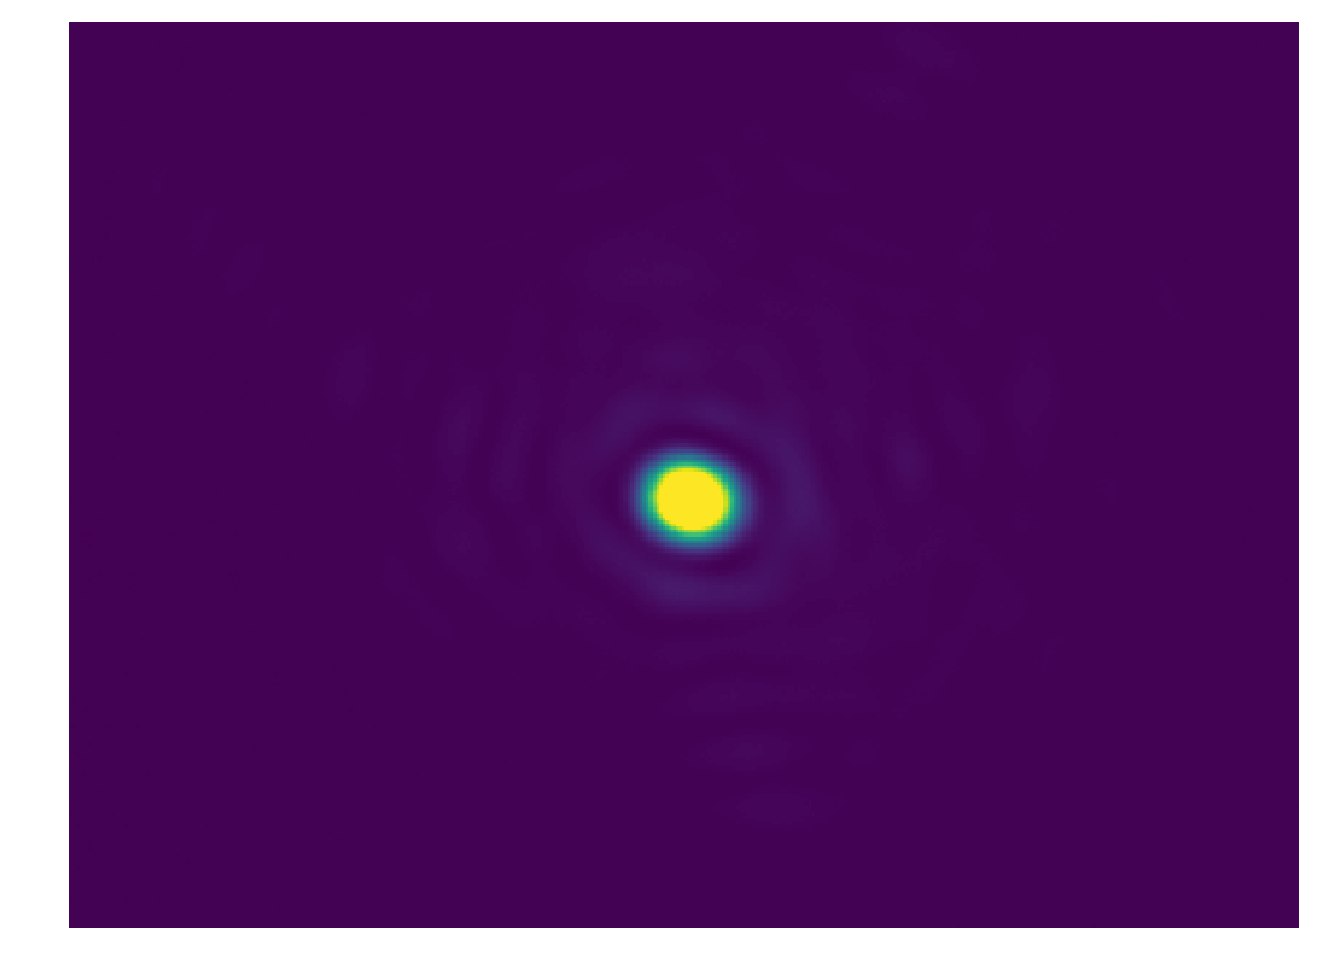
\includegraphics[width=.5\textwidth]{images/camera/profile2d.pdf}
  \caption{Image detail from the captured beam with the \gls{ccd} camera.}
  \label{fig:beamprofile:2d}
\end{figure}

The two dimensional beam profile shows the characteristical two dimensional
gaussian distribution with diffraction rings caused by beam clipping at
finite apertures as described in \cite{Hertlein2017}.

\begin{figure}[ht]
  \centering
  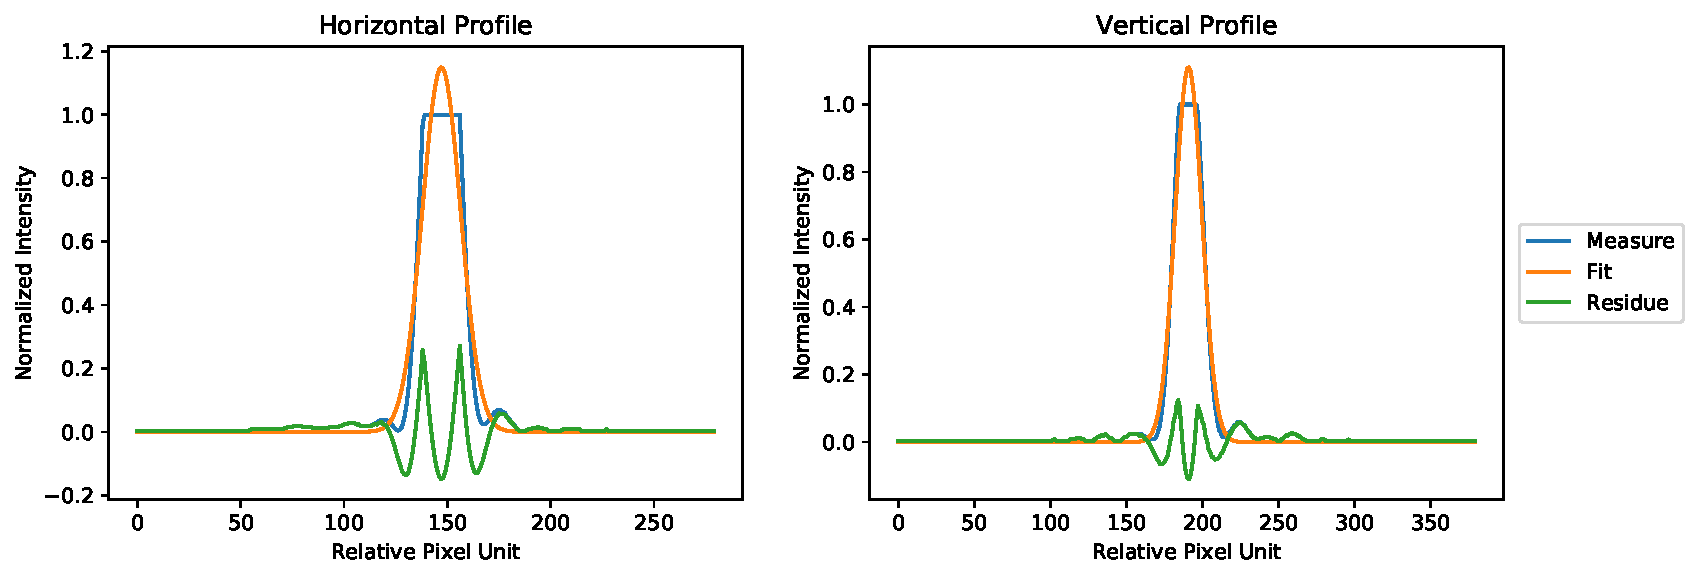
\includegraphics[width=\textwidth]{images/camera/profile1d.pdf}
  \caption{1D horizontal and vertical profile extracted from the center of
    the image detail in \cref{fig:beamprofile:2d} with fitted gaussian curve
  and residue.}
  \label{fig:beamprofile:1d}
\end{figure}

By inspecting the one dimensional profiles with fitted gaussian and residue
we again confirm conclusions drawn in \cite{Hertlein2017}. The clipped top
of the measured intensity originates from the saturated pixels of the
\gls{ccd} camera and can be ignored. We further observe a slight assymmetry
at the diffraction rings. Overall the shown profiles can be considered to
confirm a good alignment.

\chapter{Measurements}

% computer -> dds
%          -> scope
%          -> trigger
%          <- scope

\section{Electronics}

\subsection{Signal Source}

\subsection{Signal Amplifier}

% network analyzer (frequency dependence amplification)
% chirp signal deviation from ideal

\subsection{Intensity Control}

% test of long time stability

\section{Acousto-Optics}

\subsection{1D Intensity Distribution}

% H removed, V sweep (H in V position, vice versa)
% V removed, H sweep (V in H position, vice versa)

% H constant with V sweep
% V constant with H sweep

% amplitude modulation

\subsection{2D Intensity Distribution}

% without amplitude modulation
% with amplitude modulation

\chapter{Intensity Optimization}

\chapter{Conclusion}

\section{Summary}

\section{Future Outlook}

\section{Further Applications}


\printglossaries
\listoffigures
\listoftables
\printbibliography

\appendix
\chapter{Electronics}

\section{Trigger Hub}
\label{app:electronics:trigger_hub}

The trigger hub is driven by a \SI{3.3}{\volt} input signal and a
\SI{5}{\volt} voltage source. The input signal is amplified to drive four
\gls{ttl} inputs through use of the \gls{sn74128} \cite{SN74128} line driver.
Furthermore the hub is designed to be mounted on the \gls{bbb} which itself
provides the trigger network interface.

\begin{figure}[h]
  \centering
  \captionsetup{width=.8\textwidth}
  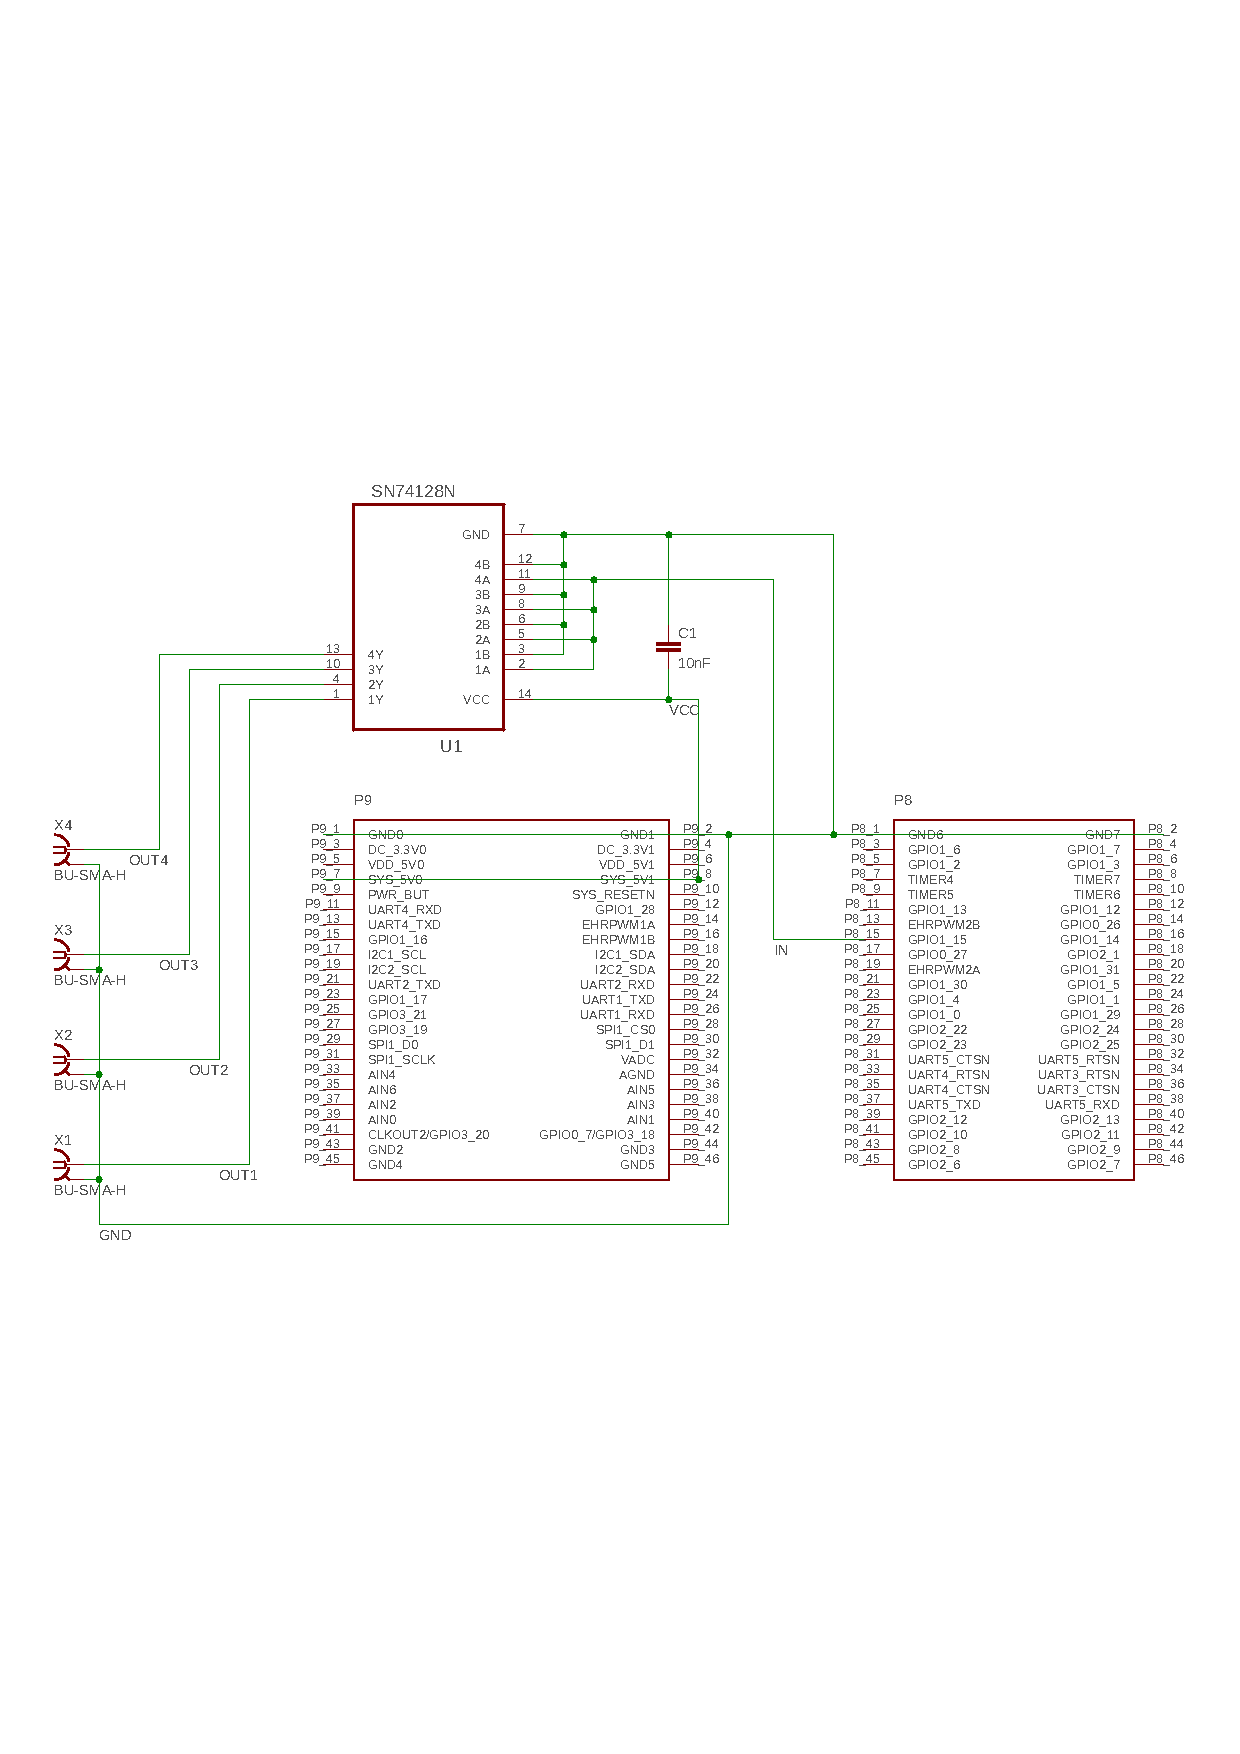
\includegraphics[width=\textwidth]{images/circuits/line-driver/schematic.pdf}
  \caption{Elecronic circuit schematics of the trigger hub. The
    \SI{3.3}{\volt} input signal is amplified by the \gls{sn74128} line
    driver and outputed to four \gls{sma} connectors.}
\end{figure}

The \gls{sn74128} exposes four independent outputs $Y$, each is driven by a
two-input ($A$ and $B$) with NOR ($\overline{A+B}=Y$) logic. As our objective
is to forward rising edge trigger signals we pulled all four $B$ to low by
connecting them with \gls{gnd}. The four $A$ where connected together with
the input signal. The input signal has to transition from $1$ to $0$ in order
to signal a rising edge trigger signal.

\begin{listing}[h]
  \inputminted[xleftmargin=.2\linewidth]{javascript}{scripts/trigger.js}
  \captionsetup{width=.6\linewidth}
  \caption{\gls{bbb} script that starts a \gls{http} server to listen for
requests on which to trigger a rising edge signal. On execution it pulls the
signal \gls{gpio} to high. The request callback then pulls the \gls{gpio} to
low for one \SI{1}{\milli\second}.}
\end{listing}

Using the \gls{bbb} makes it easy to write scripts that communicate with
other devices over the \gls{lan}. We used the bonescript library to access
the \gls{gpio} interface as it is pre-installed on the \gls{bbb}.

\begin{figure}[h]
  \centering
  \begin{minipage}{.40\textwidth}
    \centering
    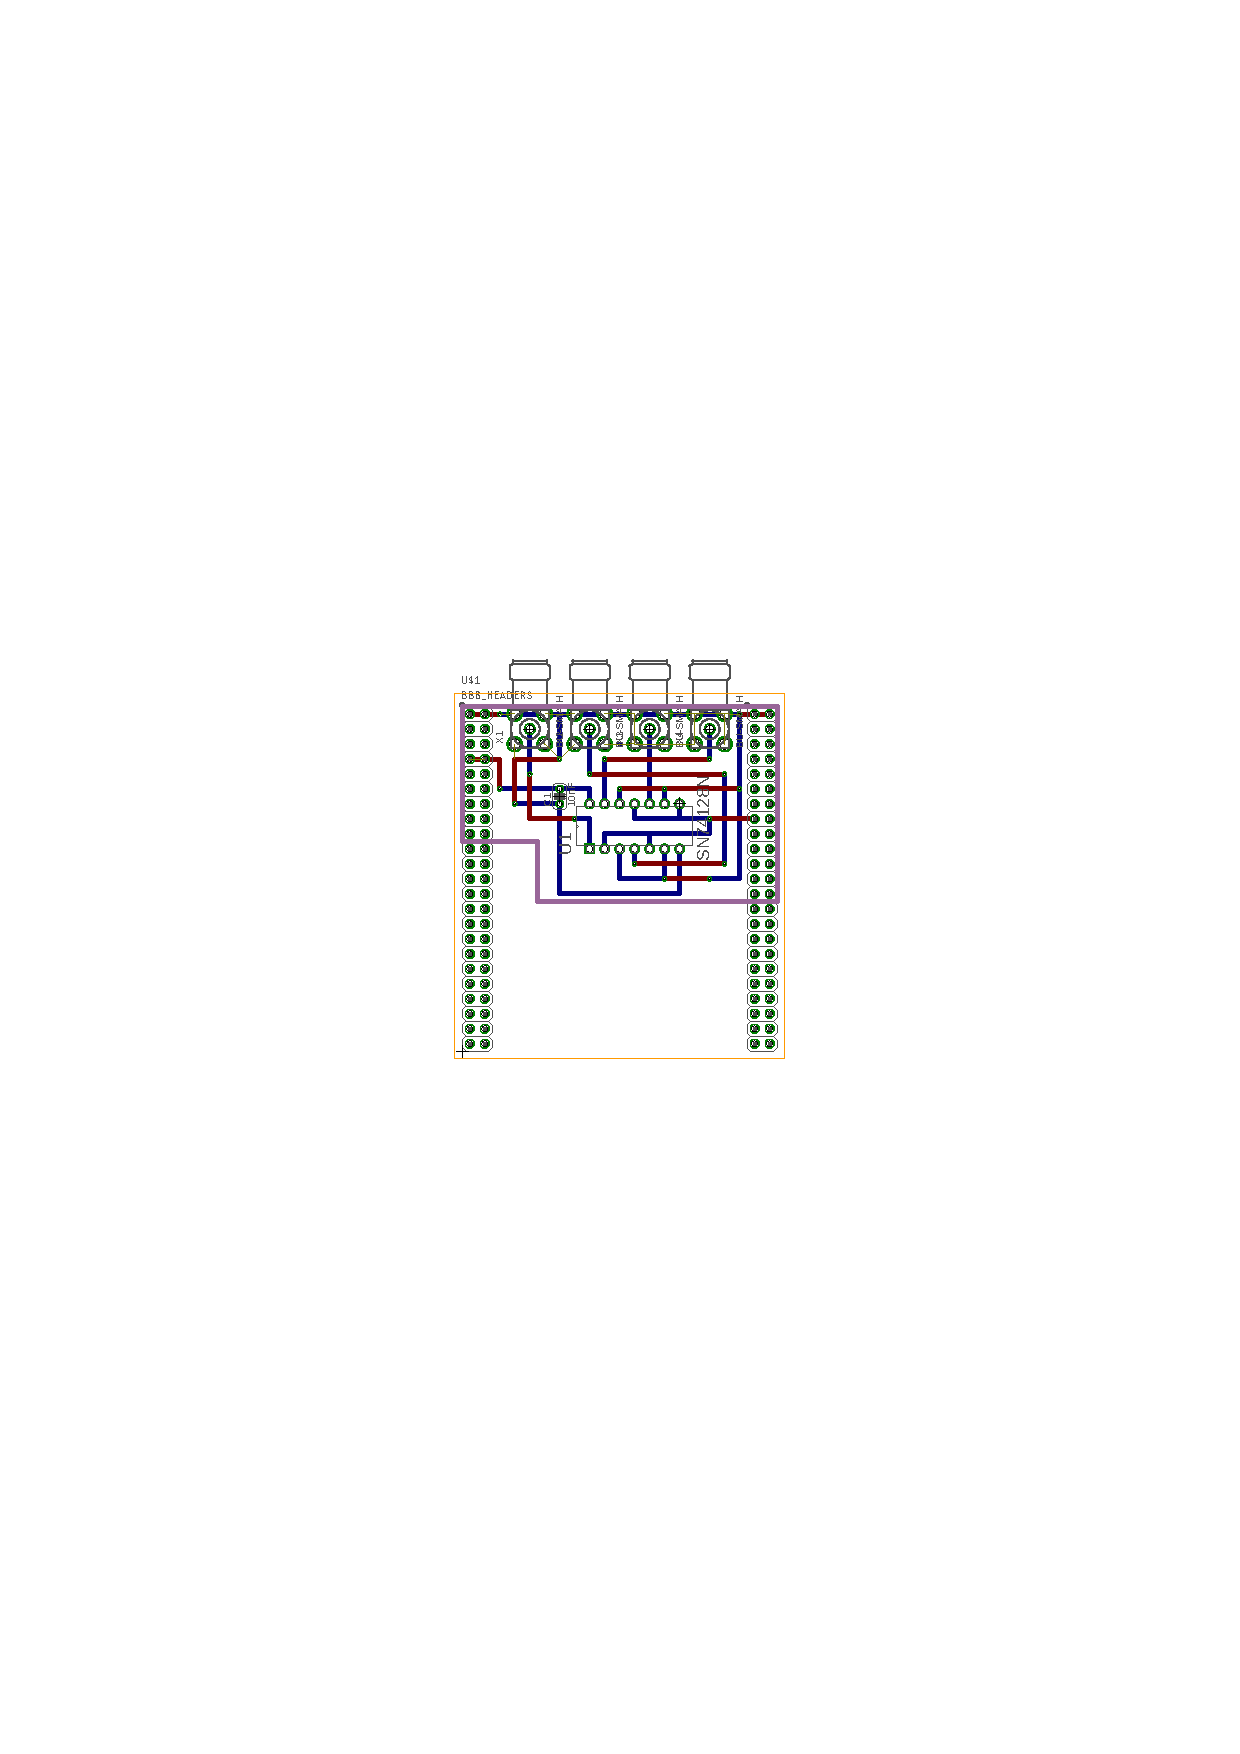
\includegraphics[width=\linewidth]{images/circuits/line-driver/layout.pdf}
    \captionsetup{width=\linewidth}
    \caption{Board layout of the trigger hub. The source amplifier is designed
to fit on top of the \gls{bbb} expansion headers.}
  \end{minipage}
  \begin{minipage}{.50\textwidth}
    \centering
    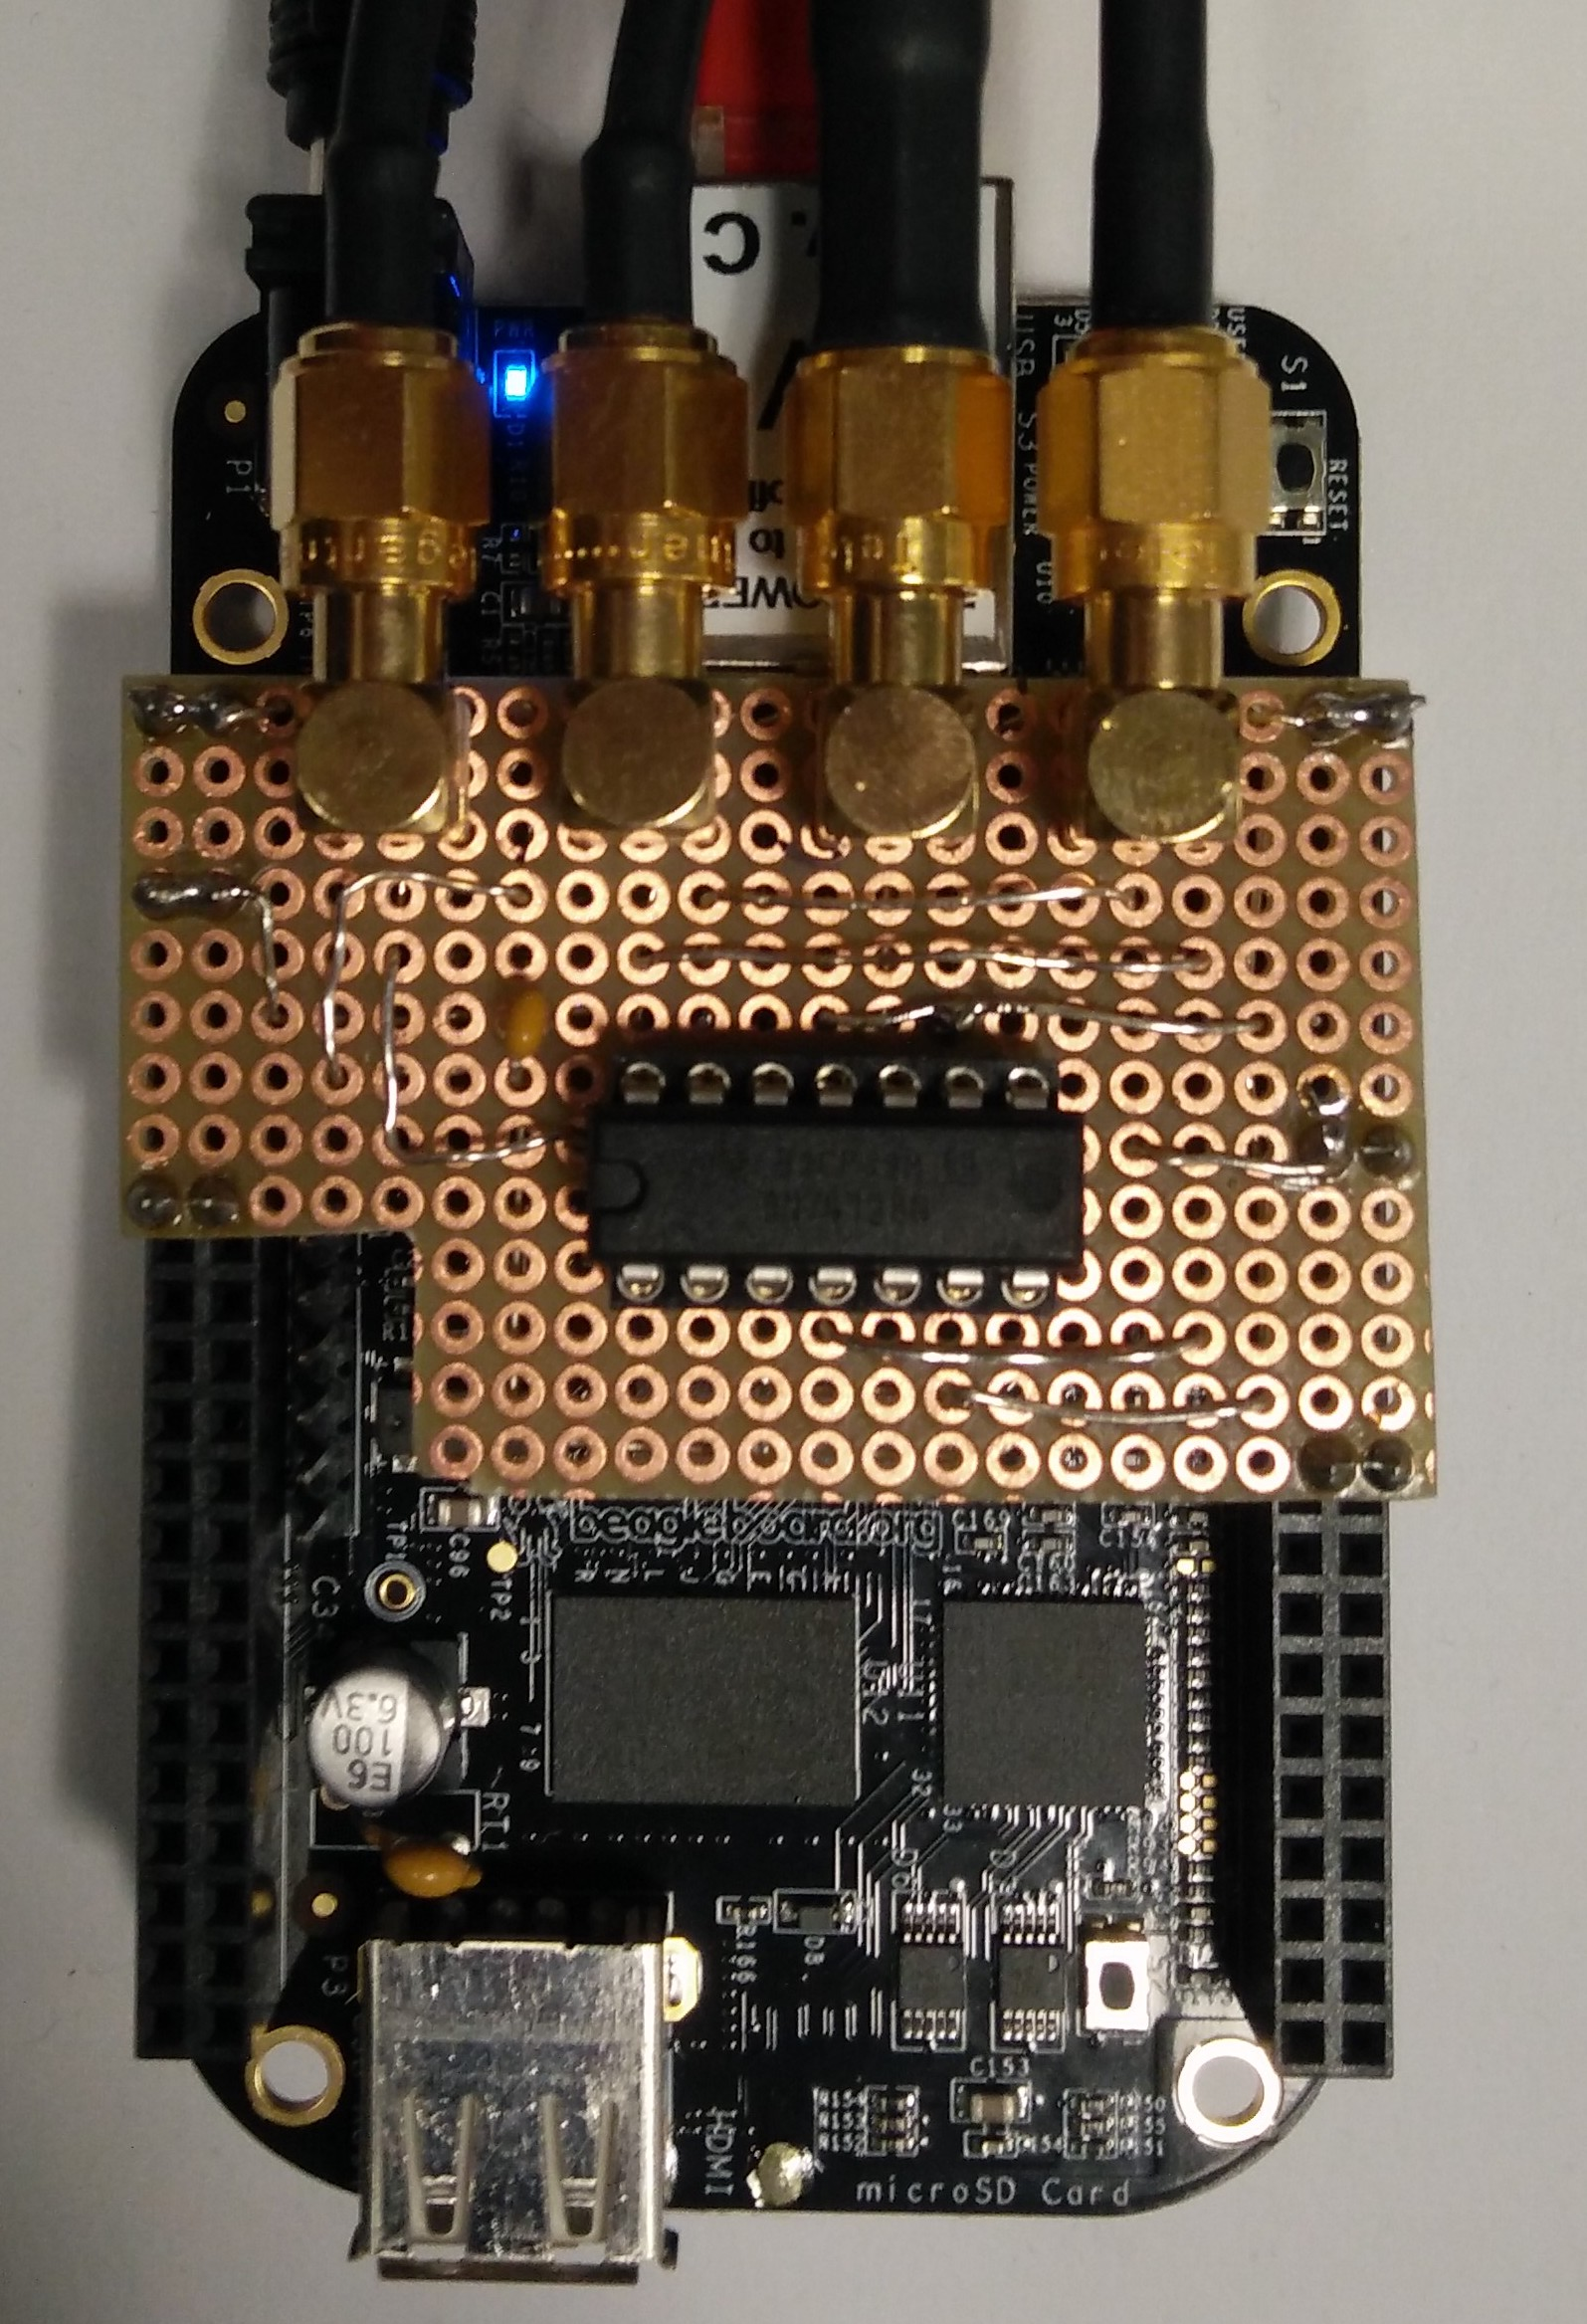
\includegraphics[width=.6\linewidth]{images/circuits/line-driver/board.jpg}
    \captionsetup{width=.8\linewidth}
    \caption{Picture of the trigger hub on the \gls{bbb}. The \gls{bbb} is
connected with the \gls{lan} via cable. The trigger hub forwards the signal
to the oscilloscope, the camera and the two \gls{dds}.}
  \end{minipage}
\end{figure}


\end{document}
